\documentclass[../document.tex]{subfiles}
 
\begin{document}


\subsection{Redox-Reaktionen}
Eine Redoxreaktion (eigentlich: Reduktions-Oxidations-Reaktion) ist eine chemische Reaktion, bei der ein Reaktionspartner Elektronen auf den anderen überträgt

\subsubsection{Galvanische Zelle}
auch galvanisches Element oder galvanische Kette genannt, ist eine Vorrichtung zur spontanen Umwandlung von chemischer in elektrische Energie.

Jede Kombination von zwei verschiedenen Elektroden und einem Elektrolyt bezeichnet man als galvanisches Element und sie dienen als Gleichspannungsquellen.

Es gibt drei Gruppen von galvanischen Zellen:
\begin{itemize}
	\item \textbf{Primärzellen}, auch Batterie genannt. Nach dem Zusammenfügen kann sie nur einmal eintladen und nicht wieder aufgeladen werden. 
	\item \textbf{Sekundärzellen}, auch Akkumulator (kurz: Akku) genannt. Sie können nach einer Entladung durch eine der Entladung gegenläufige Stromrichtung wieder aufgeladen werden. Dieser Vorgang ist aber durch Verschleiß begrenzt (Zyklenzahl). Im Vergleich zu Primärzellen ist die Energiedichte geringer.
	\item \textbf{Tertiärzellen}, auch Brennstoffzellen gennannt. Bei diesen Zellen wird die chemische Energie nicht in der Zelle selbst gespeichert sondern kontinuierlich von außen zugeführt. Dadurch wird ein im Prinzip zeitlich unbeschränkter Betrieb ermöglicht.
\end{itemize}

Du Funktion der galvanischen Zelle: Reduktion und Oxidation laufen räumlich getrennt ab. Durch verbinden der beiden Halbzellen mit einem Ionenleiter und einem Stromleiter wird der Stromkreis geschlossen.

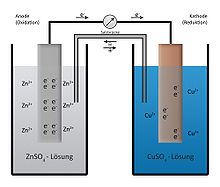
\includegraphics{images/daniell_element} %TODO: own graphics because of copyright reasons

Die Spannung des elektrischen Strom hängt ab von der:
\begin{itemize}
	\item Art des Metalls (elektrochemische Spannungsreihe)
	\item Konzentration in der Lösung
	\item Temperatur
\end{itemize}


\subsubsection{Korrosionsschutz}

Eine Opferanode ist ein Stück unedles Metall, das an Geräten und Fahrzeugen zum Schutz von Funktionsteilen aus edleren Metallen (z.B.: Eisen, Stahl, Stahlbeton oder Messing) gegen Kontaktkorrosion.

Dadurch das das unedlere Metall (oft Magnesium oder Zink) zur Anode wird findet dort die Oxidation statt. Während die Kathode geschützt wird oxidiert die Opferanode und muss deswegen regelmäßig ausgetauscht werden um fortlaufenden Schutz zu ermöglichen.

\subsection{Anorg. Rohstoffe \& Produkte}
\subsubsection{H+Brennstoffzelle}


\subsubsection{Silizium}

Silizium kommt in der Natur nicht als reines Element vor. Man findet es meist oxidiert in Form von z.B. Sand. In reinem Zustand ist es dunkelgrau, kristallin, spröde und leicht zu pulverisieren. Es wird 

%Zonenschmelzen
%Halbleiter n und p + Andwendung
\subsubsection{Kohlenstoff Modifikationen}

\end{document}
